\documentclass{Class/class}
\usepackage[utf8]{inputenc}
\usepackage[T1]{fontenc} 
\usepackage{subcaption}

\usepackage{color}
\usepackage{lipsum}
\usepackage{array}
\usepackage{amsmath}
\usepackage{float}
\usepackage{listings}     % Package for including code snippets
\usepackage{xcolor}       % For custom colors
\usepackage{tikz}
\usepackage{graphicx}
\usepackage{comment}


% Define a new language for your programming language
\lstdefinelanguage{Bleach}{
    % Define keywords
    morekeywords={and, break, class, continue, do, elif, else, false, for, function, if, inherits, lambda, let, method, nil, or, print, return, self, super, true, while},
    % Define other keywords (e.g., types or built-ins) with different styles
    morekeywords=[2]{std::chrono::clock, std::io::readLine, std::io::print, std::io::fileRead, std::io::fileWrite,
    std::math::abs, std::math::fmod, std::math::log, std::math::pow", std::math::sqrt, std::random::random,
    std::utils::ord, std::utils::numToStr, std::utils::strToNum, std::utils::strToBool, std::utils::strToNil},
    % Define comments
    comment=[l]{//}, % Line comment with //
    morecomment=[s]{/*}{*/}, % Block comment between /* and */
    % Define string delimiters
    morestring=[b]", % Strings are enclosed in double quotes
    % Styling for different parts
    keywordstyle=\color{blue}\bfseries,   % Style for keywords (bold blue)
    keywordstyle=[2]\color{teal},         % Style for secondary keywords (teal)
    commentstyle=\color{gray}\itshape,    % Style for comments (italic gray)
    stringstyle=\color{red},              % Style for strings (red)
    numberstyle=\tiny\color{gray},        % Line numbers style (tiny gray)
    backgroundcolor=\color{white},        % Background color (optional)
    showstringspaces=false,               % Don't show spaces in strings
}

\lstset{
    language=Bleach, % Change to your language
    basicstyle=\ttfamily\small,
    keywordstyle=\color{blue},
    commentstyle=\color{gray},
    stringstyle=\color{red},
    numberstyle=\tiny\color{gray},
    numbers=left,
    stepnumber=1,
    breaklines=true,
    frame=single,
}

\newcommand{\Fix}[1]{[\textbf{TODO}: {\color{red} #1}]}
\newcommand{\atencao}[1]{[\textbf{!!ATTENTION!!}~{\color{red} #1}]}
\newcommand{\lmt}[1]{[\textbf{Leopoldo}:~{\color{orange} #1}]}


\usepackage[linesnumbered,ruled,vlined]{algorithm2e}
\usepackage{csquotes}
\begin{document}
\newcommand{\numprotocolos}[1][16]{#1 }

\frontmatter

\newpage
\begin{titlepage}
    \thispagestyle{empty}
    \begin{center}
    \includegraphics[width=3cm]{Figures/logoufpe.jpg}
  \large
  \\Universidade Federal de Pernambuco
  \\Centro de Informática
  \vskip 25mm
  Bachelor's Degree in Computer Engineering
  \vskip 45mm
  \begin{minipage}{160mm}
    \begin{center}
      \textbf{Bleach: A programming language aimed for teaching Compilers}
      \vskip\baselineskip
      Victor Miguel de Morais Costa
      \vskip\baselineskip
      Undergraduate Thesis
    \end{center}
  \end{minipage}\\
  \vfill
  Recife, Pernambuco\\
  October , 2024
  \end{center}
\end{titlepage}
\newpage
\thispagestyle{empty}
    \begin{center}
    \large
    Universidade Federal de Pernambuco\\
    Centro de Informática\\
    \vskip 25mm
    Victor Miguel de Morais Costa
    \vskip\baselineskip
    \textbf{Bleach: A programming language aimed for teaching Compilers}
  \vskip 58mm
  \begin{flushright}
    \begin{minipage}{100mm}
    \small{
    Work presented to the Undergraduate Course in Computer Engineering at the Informatics Center of the Federal University of Pernambuco as a partial requirement to obtain the Bachelor's degree in Computer Engineering.}
    \vskip2\baselineskip
    \small{\textbf{Concetration Area: Compilers, Interpreters, Programming Languages} }
    \newline \small{\textbf{Advisor: Leopoldo Teixeira} }
    %\newline \small{\textbf{Co-orientador:} }
    \end{minipage}
  \end{flushright}
  \vfill
  Recife, Pernambuco\\
  October, 2024
  \end{center}
\input{dedication.tex}
\thispagestyle{empty}
\begin{spacing}{1.0}
\chapter*{Acknowledgments}

Andrea,

Alvaro,

Maria Dolores,

Laura,

Leopoldo Motta Teixeira,

Fernando Castor, Gustavo Carvalho,

Daniel Perazzo, Fernando Macedo, Lucas Ambrosio, Matheus Teotônio, Riei Joaquim, Victor Hugo, Victor Ximenes, Zênio Ângelo

José Carlos da Silva Cruz, Pedro Nogueira Coutinho, Zilde Souto Maior Neto

José Victor Silva Cruz, Lucas Santana, Marcos Oliveira,

Cintia,

Noriaki Kubo,
    
\clearpage
\end{spacing}
\newpage
\thispagestyle{empty}
  ~\\\vfill
\begin{flushright}
    \begin{minipage}{0.6\textwidth}
      \begin{flushright}
        \begin{quote}
           \textit{``The ocean is full 'cause everyone's crying \newline
           The full moon is looking for friends at high tide \newline
           The sorrow grows bigger when the sorrow's denied \newline
           I only know my mind \newline
           I am mine \newline
           \newline
           And the meaning, it gets left behind \newline
           All the innocence lost at one time \newline
           Significant, behind the eyes \newline
           There's no need to hide \newline
           We're safe tonight \newline
           \newline
           And the feelings that get left behind \newline
           All the innocence broken with lies \newline
           Significance, between the lines \newline
           We may need to hide \newline
           \newline
           And the meanings that get left behind \newline
           All the innocence lost at one time \newline
           We're all different behind the eyes \newline
           There's no need to hide, yeah"} 
        \end{quote}
        \vskip.2\baselineskip%
        --- "I am Mine", Pearl Jam, 2002
      \end{flushright}
    \end{minipage}
\end{flushright}


%\maketitle

\thispagestyle{empty}
\begin{spacing}{1.0}
\chapter*{Resumo}
Nos cursos de bacharelado em Ciência da Computação ou Engenharia da Computação, espera-se que os alunos tenham contato com uma disciplina de Compiladores de nível introdutório. Devido à grande amplitude e complexidade dos temas abordados nesta disciplina, os professores responsáveis tendem a conduzi-lá sob um ponto de vista mais teórico. 

Esta abordagem costuma proporcionar aos alunos uma compreensão mais profunda dos conceitos fundamentais desta área e prepará-los melhor para uma carreira orientada para a pesquisa científica. No entanto, tende a limitar a experiência prática dos conceitos ensinados, fazendo com que os alunos muitas vezes se sintam desconectados das aplicações dessa área, causando um menor engajamento e motivação entre estes. Diante disso, desde a década de 90, novas metodologias, que mesclam teoria e prática, começaram a surgir. Na maioria delas, os alunos devem implementar um compilador ou um interpretador para uma linguagem de programação de fins didáticos, normalmente definida pelo professor responsável.

Devido às desvantagens mencionadas da abordagem tradicional e às limitações que algumas das linguagens propostas na abordagem mista apresentam, a proposta atual visa apresentar uma nova linguagem de programação chamada Bleach, juntamente com uma implementação de seu interpretador. Tal linguagem pretende ser utilizada como ferramenta em disciplinas introdutórias de Compiladores que optem por seguir uma abordagem de ensino mais voltada para a prática incremental, priorizando a flexibilidade e objetivando solucionar, ou pelo menos mitigar, as desvantagens de ambas as abordagens mencionadas.

\textbf{Palavras-chave:} Compiladores; C++; Educação; Software Educacional; Interpretadores; Linguagens de Programação.
        
\clearpage
\end{spacing}
\chapter*{Abstract}
\begin{spacing}{1.0}
In Bachelor's degrees in Computer science or Computer engineering, students are expected to have contact with an introductory-level Compilers course. Due to the large breadth and depth of topics in this subject, professors and instructors tend to conduct it from a more theoretical point of view. 

This approach tends to provide students a deeper understanding of the fundamental concepts of this field and better prepare them better for a research oriented career. However, it tends to limit the hands-on experience of the taught concepts, making students often feel disconnected from real-world applications of this area, causing less engagement, excitement and motivation among them. Given this, since the 90s, new methodologies, which combined theory and practice, began to emerge. In most of them, students we required implement a compiler or an interpreter for a programming language for teaching purposes, normally defined by the responsible professor or instructor.

Due to the aforementioned disadvantages of the traditional approach and the limitations that some of the proposed programming languages in the mixed approach present, this proposal aims to present a new programming language called Bleach along with an implementation of its interpreter. This language is intended to be used as a tool in introductory-level Compilers courses whose responsible professors opt to follow a teaching approach more focused on incremental practice, prioritizing flexibility and aiming to solve, or at least mitigate, the disadvantages of both mentioned approaches.



\textbf{Keywords:} Compilers; C++; Education; Educational Software; Interpreters; Programming Languages.  

\end{spacing}
\listoftables
\listoffigures
\tableofcontents

\mainmatter

\chapter{Introduction} \label{cap:introduction}

\begin{displayquote}
    \begin{center}
        \textit{``If you were to give me wings, I would fly for you. Even if this entire land were to sink underwater. If you were to give me a sword, I would stand up and fight for you. Even if the entire sky were to pierce you with its light.''}
    \end{center}
\end{displayquote}

\begin{flushright}
   \textit{-- TITE KUBO}
\end{flushright}
\chapter{Theoretical Review} \label{Cap:theoretical_review}

\begin{displayquote}
    \begin{center}
        \textit{``Do not live bowing down. Die standing up.''}
    \end{center}
\end{displayquote}

\begin{flushright}
   \textit{-- TITE KUBO}
\end{flushright}

\section{Introduction}
This chapter is dedicated to provide a literature review about the Programming Language Design and Compiler/Interpreter Implementation fields. The conceptual content presented here is heavily influenced by \cite{aho1986compilers}, \cite{cooper2022engineering} and \cite{nystrom2021crafting}.

\section{What is a Compiler and How does it work?}
To simply put it simple, a compiler is a software whose responsibility is to translate a program written in a certain programming language into a another program written in another one, without modifying the meaning of the original program, that is, its semantics. However, despite this simple description, compilers are usually complex and large software systems composed of several components which interact with each other during the mentioned translation process, commonly known as compiling.

The importance of compilers in both computer science and real-world applications is immeasurable. The key points below illustrate some of the most prominent impacts of this creation:

\begin{itemize}
    \item \textbf{Bridging High-Level Languages to Machine Code:} As previously mentioned, the purpose of a compiler is the translation between programs written in different programming languages. Usually, in practice, such translation happens from a high-level programming language, commonly more human-readable and that provides several abstractions, into a programming language that is closer to the hardware and, therefore, more machine-readable. Given this fact, it is safe to say that a compiler provides several layers of abstractions that allow developers to build complex software that impact people's life around the world since its conception.
    
    \item \textbf{Impact on Portability:} One of the major features of compilers is their portability. In practice, this means that code once a program, written in a high-level programming language, passes through the compiling process, the resulting machine-code can be used in different hardware platforms by simply targeting different machine architectures, such as: x86, ARM, RISC-V, MIPS and others. This allows the same code base to be re-used in independent systems without the need to rewrite the code base in order to target each different architecture.
    
    \item \textbf{Programming Languages Evolution:} In the current context, it is crucial to reiterate that compilers and programming languages are deeply tied. In practice, the evolution of one serves as a trigger to the evolution of the other and vice-versa. Compilers permit language designers to experiment on new ideas that cross different programming paradigms, such as the procedural, object-oriented, functional, aspect-oriented, concurrent and several others. Furthermore, the evolution of existing programming languages and creation of new ones may allow the enhancement of existing compilers and creation of new ones for niche areas.
    
    \item \textbf{Impact on Software Development:} Without the existence of compilers, the development of software applications would become far more difficult since there would be no bridge uniting codebases written in high-level languages and hardware systems where such codebases are executed. Therefore, this would limit the growth of technology-based companies.
\end{itemize}

Given the impacts emerged from the creation of compilers, now it is time to take a deep dive into how this particular type of software works.

As already explained, a compiler is a complex software system and due to this, must be structurally organized in components responsible for executing a single task in the compiling procedure. According to \cite{cooper2022engineering}, compilers are being implemented since 1955. During these early years of development, a compiler was viewed as a tool that had to understand the program written in the source language and translate it, without altering its meaning, to a target architecture. The distinction between these two tasks, made computer scientist adopt the following structuring when it came down to the components of a compiler: each compiler should have a front-end and a back-end. 

In conformity with what has been exposed, the front-end was responsible for understanding the program written in the source language, while the back-end's responsibility lied on the process of mapping programs to machines. As the reader might have already thought, there must be some kind of link between the front-end and the back-end. That is where the Intermediate Representation (IR) comes in. The front-end must encode the needed information about the source program in some way, so it can be properly used by the back-end when it starts the mentioned mapping process later on. The Intermediate Representation is the entity that contains such information generated by the front-end. It is considered the definitive representation of the source code that will be transformed into machine-code by the back-end.

In short, it can be said that the front-end's responsibility is guarantee that the source code is well-formed and also translate it to the intermediate representation. On the other side, the back-end's duty is translate such intermediate representation into the machine-code of a specific machine architecture, respecting the physical limitations of the target hardware.

As the decades passed on, the process of designing and implementing a compiler became more sophisticated as the structure of such system became increasingly more complex and robust.

Shifting the focus of compilers' implementation to a classroom environment, it is safe to expect that students are capable of implementing more sophisticated compilers that have the following structure, which is not that far from those used in the industry:

\begin{figure}[H]  
  \centering
  \includegraphics[width=\textwidth, height=0.8\textheight, keepaspectratio]{Figures/Arquiteturas/CompilersDetailedPipeline.png}  
  \caption{A detailed compiler structure}
  \label{fig:comp}
\end{figure}


It is also completely plausible to simplify this task by asking the students to implement a compiler that follows the following simplified structure:

\begin{figure}[H]  
  \centering
  \includegraphics[width=\textwidth, height=0.8\textheight, keepaspectratio]{Figures/Arquiteturas/CompilersSimpliefiedPipeline.png}  
  \caption{A simplified compiler structure}
  \label{fig:Fluxograma}
\end{figure}
    
The next section is dedicated to provide an in-depth overview of each of the compiler's components from the simplified structure presented in the image above.


\section{Detailed Overview of Compiler's Components}

\subsection{Lexer}
The lexer is the first component present in the compiling process of a compiler. It is responsible for executing a process called lexing, which is also known as lexical analysis.

As earlier elucidated, the input of a compiler is the source code of a program written in a specific programming language. The content present inside the source code is viewed by the compiler as a large string, a linear sequence of characters, that has no meaning for it at all at this stage. The lexer's goal is to transform this sequence of characters that is the source code into a new representation that is more abstract from the compiler's perspective, so it can be passed on to the next component, the parser.

To perform such procedure, the lexer takes in this stream of characters and group them together forming a sequence of entities that convey the idea of a "word". These entities are called tokens.

Making an analogy to linguistics, one can say that the lexer's purpose is to group letters (characters) into words (tokens). Given this analogy, it is essential to inform the reader that, like words, tokens can have different lengths and different meanings. Some examples are listed below to better illustrate a few cases:
\begin{itemize}
    \item Single-Character Tokens: \texttt{(}, \texttt{\{}, \texttt{+}, \texttt{-}, \texttt{*}, \texttt{/}, etc.
    \item Double-Character Tokens: \texttt{==}, \texttt{!=}, \texttt{>=}, \texttt{<=}, etc.
    \item Multi-Character Tokens: \texttt{123} (a number literal), \texttt{"hello"} (a string literal), \texttt{true} (a boolean literal), \texttt{aVariable} (an identifier), etc.
\end{itemize}

It is also important to mention that certain characters have no meaning for the lexer during the lexical analysis and, therefore, are completely ignore in the process, such as: whitespace characters and characters that represent comments in the programming language in which the source file was written.

By the end of the lexical analysis, the sequence of characters is transformed into a sequence of tokens by following the syntax rules of the source programming language.

The figure below shows, in an simple example, the input and the output of this component:

\newpage

\begin{table}[h!]
    \centering
    \begin{tabular}{|c|c|c|c|c|c|c|c|c|c|c|c|c|c|c|c|c|c|c|c|c|}
        \hline
        l & e & t &  & a & v & g &  & = & ( & m & i & n & + & m & a & x & ) & / & 2 & ; \\
        \hline
    \end{tabular}
\end{table}

\begin{figure}[h!]
  \centering
  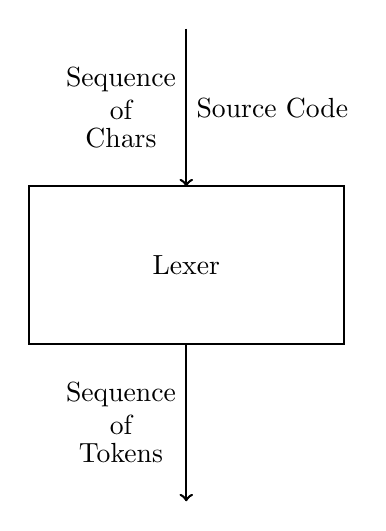
\begin{tikzpicture}
    % Draw the boxes
    \draw[thick] (0, 0) rectangle (4, 2);
    
    % Labels inside the boxes
    \node at (2, 1) {Lexer};

    % Input and output arrows
    \draw[->, thick] (2, 4) -- (2, 2) node[midway, left] {\shortstack{Sequence\\ of\\ Chars}};
    \draw[->, thick] (2, 4) -- (2, 2) node[midway, right] {\shortstack{Source Code}};
    \draw[->, thick] (2, 0) -- (2, -2) node[midway, left] {\shortstack{Sequence\\ of\\ Tokens}};
    \draw[->, thick] (2, 0) -- (2, -2) node[midway, left] {\shortstack{ }};
  \end{tikzpicture}
\end{figure}

\begin{table}[h!]
    \centering
    \begin{tabular}{|c|c|c|c|c|c|c|c|c|c|c|}
        \hline
        let & avg & = & ( & min & + & max & ) & / & 2 & ; \\
        \hline
    \end{tabular}
\end{table}

\begin{figure}[H]  
  \caption{Input and Output of a Lexer}
  \label{fig:lexer}
\end{figure}

As seen in the example above, the lexer receives a sequence of characters, which represents the raw source code, and gives as the result a series of chunks of characters called tokens. Making another analogy with linguistics, one can think of tokens as the "words" and  the "punctuation" that constitutes a programming language.

Going further, it is also possible to say that the lexer's job is execute a traversal through the sequence of characters received and group such characters into the smallest sequences that represent something in the source programming language. Each of these resulting sequences of grouped characters is called a lexeme.

Therefore, in the example presented above, the sequence of lexemes produced from analyzing the sequence of characters received as input was: \texttt{let}, \texttt{avg}, \texttt{=}, \texttt{(}, \texttt{min}, \texttt{+}, \texttt{max}, \texttt{)}, \texttt{/}, \texttt{2}, \texttt{;}

In conclusion, lexemes are just raw substrings presented in the source code.

However, a token is much more than a lexeme. It generally contains other pieces of information that are useful in further stages of the compiling process and also in error report.

Usually, each token has a token type associated. For example, the lexeme \texttt{2} usually has \texttt{NUMBER} as its token type, while \texttt{+} often has \texttt{PLUS} as its token type. In this context, it is relevant to highlight that the amount of token types in a programming language basically depends on the amount of keywords (reserved words) that the language has, the amount of operators at the user's disposal, possibilities of literal values of different data types and, finally, the quantity of delimiters and separators.

Certain types of lexemes have literal values associated with them. numbers, booleans and strings, for example, fall into this category. In these cases, the lexer is able to convert the textual representation of the value into the living runtime entity that might be used by the compiler on later stages of the compiling process.

Last but not least, a compiler must also report errors when it encounters a lexical error during the lexing process, such as: an invalid number literal, an unterminated string, an invalid character that does not follow certain rules of the programming language. In order to report these errors, it is desired that the compiler display as much information as possible to the user about what went and, most importantly, where things went wrong. Having this in mind it is essential to store information about the location of each lexeme in the source code (the line it has appeared and, if possible, its column also).

Now it is time to analyze the functioning of a lexer from an implementation perspective.

\subsection{Parser}
The Parsing phase of a compiling/interpreting process, also known as Syntax Analysis,

\subsection{Static Analyzer}
The Static Analysis phase of a compiling/interpreting process

\subsection{Intermediate Representation (IR) Generator}
After the previous phases have been executed

\subsection{Optimizer}
The Optimization phase of a compiling/interpreting process

\subsection{Code Generator}
The Code Generation phase of a compiling process


\subsection{Virtual Machines}
Virtual Machines are 

\subsection{Runtimes}
Runtimes are

\section{Shortcuts and Alternate Routes}
This section is dedicated to present an overview of a few ad-hoc strategies that might be used when implementing a programming language.

\subsection{Single-Pass Compilers}
A Single-Pass Compiler

\subsection{Tree-Walk Interpreters}
A Tree-Walk Interpreter

\subsection{Transpilers}
A Transpiler


\section{Compilers and Interpreters}


\chapter{Context and Purpose} \label{cap:metodologia}

\begin{displayquote}
    \begin{center}
        \textit{``I wonder if I can keep up with... the speed of a world you're not in.''}
    \end{center}
\end{displayquote}

\begin{flushright}
   \textit{-- TITE KUBO}
\end{flushright}

\section{Introduction}
This chapter is dedicated to provide the historical context behind how the way of teaching undergraduate Compilers courses evolved since the 70s, as well as a brief overview of surveys that demonstrate the positive impact that more practice-orient approach brings to students. Such factors are what motivated the creation of the Bleach programming language. Furthermore, a revisit and deepening regarding the purpose of Bleach will also be made. Then, an analysis about how Bleach distinguishes itself from other proposed programming languages that also aim to solve its same issue will be presented. In the end, the chapter will provide a detailed description about the context Bleach is inserted in, which includes: the target audience, educational environment, typical use cases and the educational benefits provided by it.

\section{Historical Context of Undergraduate Compilers \newline Courses}
Looking back, it can be said that the way of teaching an undergraduate Compilers course evolved as follows:

During the 1970s, undergraduate Compilers courses used to have a heavy focus on the theoretical aspects of the field, such as: formal languages, automata theory, lexing techniques and parsing techniques. During that period, access to computational resources were still scarce, even in an academic environment. However, students were still able implement toy compilers in different tastes of Assembly or in an early high-level language like Fortran \cite{fortran_official_website}. Still, the pillars of this course emphasized a deep understanding of the theoretical and formal aspects mentioned above.

In the 1980s, even though the focus of these courses remained rooted in theoretical aspects (lexical analysis, syntax analysis and the fundamental of code generation and optimization), a gradual shift from theory to practice started to happen. Thanks to the spread of languages like C \cite{kernighan1988c}, C++ \cite{strousrup2000c++} and Pascal \cite{wirth1971programming}, more practical implementations of compilers were allowed to be made. Therefore, courses started to add more practical projects. In such projects, students were usually asked to write a compiler (or parts of one) in these new languages. Last, but not least, the rise of UNIX \cite{ritchie1978unix}, Lex \cite{lesk1975lex} and Yacc \cite{johnson1975yacc} allowed students to implement components of a compiler with more ease. This improvement led to more sophisticated course projects.

In the 90s, such courses had already become more oriented to hands-on experience thanks to the improvements achieved in the previous decade. The birth of languages like Java \cite{java_17_official_specification} and the increase in computational power of personal computers allowed students to tackle more complex compiler projects. Courses started to assign to students more complicated tasks like the implementation of entire compilers for small languages or significant compiler components, such as code generators and optimizers. Moreover, the textbook \cite{aho1986compilers}, popularly known as "The Dragon Book", became the standard reference in this field.

In the 00s, this trend of giving more focus to the practical experience went on, with a focus on real-world applications and the use of modern programming languages. Furthermore, courses began to add more advanced topics to their syllabus, such as just-in-time compilation, garbage collection, and runtime environments. It's safe to say that the way of teaching Compilers became more holistic, covering not just compiler theory and implementation but also language design and performance optimization. During this period, Alfred Aho published \cite{aho2008teaching}, an article in which he reflects on how the way of teaching undergraduate Compilers courses has evolved through the years and also how he changed his way of teaching such course. According to him, it is still possible to teach it in a way that provides educational benefits and satisfaction to the students. The latest approach adopted by him consisted on presenting the basics of the most important topics (lexical analysis, parsing, semantic analysis, intermediate code generation, runtime environments, resource management and target code generation). At the same time, Aho asked his students to implement a compiler and provided the specifications of the source and target languages for the compiler they were implementing. He also noticed that the students weren't excited about implementing someone else's language. Thus, he took a bold move and assigned his students the task of working in smalls team to define their own
language and then build a compiler for it. Such approach, according to him, made the students much more engaged and excited.

Finally, in the 2010s and 2020s, the teaching of this course continued the trend of emphasis on balancing theory and practice. Such factor influenced the way Compilers course were taught, as professors and instructors began to integrate more diverse and flexible learning materials, including video lectures, interactive simulations, and online coding platforms. Also, the COVID-19 pandemic played an important role in this change, since it forced educators to rethink how compilers could be taught in a remote manner, which led to rise of new assisting tool like virtual laboratories, collaborative coding environments and online assessment tools. Consequently, such courses became more modular, allowing students to learn at their own pace and apply their knowledge in a way that felt meaningful to them.

\section{Reports on More Practical Ways of Teaching Compilers Courses}
In this section, a few reports that discuss different approach to teach an undergraduate Compilers course are presented, along with their main findings.

In 2015, Lasseter \cite{lasseter2015interpreter} proposed a new strategy to present the fundamental concepts of an undergraduate Compiler Construction course. The suggested approach defends that the concept of an Interpreter serves as an effective conceptual framework that can be used to educate students about the later stages of the compilation pipeline, specially the semantic analysis and code generation phases. As reported by the author, this line of action is useful in the way that it not only unifies the major theoretical concepts of this undergraduate course, but is also helpful when it comes to the implementation of semester-long compiler construction project. At Hobart \& William Smith Colleges, the university where Lasseter works, the undergraduate Compiler Construction course is a one-semester, upper-division elective, offered every other year. The course addresses both software engineering aspects as well as the major concepts of a traditional Compilers course (lexing, parsing, semantic analysis and code generation). Moreover, it already adopts a more practice-oriented approach where every student must present a working compiler by the end of the 15-week semester. When it comes to the course project itself, Lasseter opted to use the Tiger programming language \cite{appel1998tiger}, originally developed by Andrew Appel for his project-oriented "Modern Compiler Implementation" suite of C, ML and Java textbooks \cite{appel1997modernCompilerImplementationC}, \cite{appel2002modernCompilerImplementationJava}, \cite{appel2004modernCompilerImplementationML}. During the years in which the author was responsible for this course, he noticed a worrying pattern: Even though the students did well in the first stages of compilation (lexing and parsing), the vast majority of them started to struggle with the semantic analysis stage. According to the students, the combination of the underlying concepts of type checking, the details of the famous visitor pattern when traversing an AST and the interaction between this design pattern and a real-world semantic analysis implementation is just too overwhelming. Given this scenario, Lasseter chose to schedule individual meetings with this students where he introduced the idea of a language's interpreter as a touchstone to better explain the last two stages of the compilation pipeline. His investigation led to the fact that such approach proved to be the to be most uniformly effective among the students with whom he discussed. In light of this discovery, professor Lasseter reorganized his lectures introducing these specific compiler phases to include the interpreter structure as a reference point. Finally, he came to the conclusion that adding lectures that presented the concepts behind the interpreter framework resulted on better understanding of the students when it came down to the semantic analysis and code generation phases of the compilation process, indicating that the idea of an interpreter has a substantial educational value in this field.

In 2016, Kundra et al. \cite{kundra2016experience} proposed a novel approach called "Case-based and Project-based Learning" to teach a Compilers Design course to B.Tech third year students of a Delhi University (India) college. The responsibles for implementing such methodology based themselves in the definition of what is Traditional Learning present in \cite{altman2010workplace} and used the definition and core ideas of Case-based Learning present in \cite{golich2000abcs} in order to propose their own method. According to the authors, this proposed method combines 4 different pedagogical models, which makes this approach unique and effective: Didactic Teaching \cite{altman2010workplace}, Problem-Based Learning \cite{hmelo2004problem}, Cognitive Apprenticeship Model \cite{dennen2008cognitive} and Project-Based Learning \cite{thomas2000review}. To implement it, they divided one core project of this class into several sub-projects with the goal of improving the practical experience of the students when it came down to the task of designing a compiler. To evaluate the effectiveness of this approach, students were asked to complete a survey that grasped on their perceptions about the upsides of such method. Such survey was analyzed using the following statistical tools: frequency estimation and chi square test of association. According to the paper, the results showed that the proposed approach indeed had a positive impact on students since it enhanced their learning, critical thinking, engagement, communication skills and team work. In the end, the authors came to the conclusion that the outcome of the survey analysis proved that both Case-based and Project-based learning are suitable for teaching concepts of compilers implementation.

In 2021, Robert Nystrom, a software engineer that works at Google on the Dart language, published the "Crafting Interpreters" book \cite{nystrom2021crafting}: An extensive guide about not only implementing two different types of interpreters for Lox, a full-featured programming language designed by the author, but also a walkthrough that guides the readers on how they can design their own programming language. The book assumes that its the reader first contact with this field. Therefore, it covers each concept needed in an approachable style while also providing every line of code needed to implement the two types of interpreters covered. As the author himself admits in the first chapter of the book, "Crafting Interpreters" is not meant to be as rigorous as other references, such as \cite{aho1986compilers} or \cite{cooper2022engineering} when it comes to the theoretical foundation of programming languages. Instead, as suggested earlier, its purpose is to be lighter in theory, while still introducing the history and core concepts of programming languages implementation. Moreover, the author stands by the point of view that the best way of learning a new subject is by practicing and experimenting. He even says that his goal is that every reader finish his book with a solid intuition about how real programming languages work. The book also aims that the reader will feel more comfortable when reading more advanced and theoretical books later on, such as \cite{aho1986compilers}, \cite{cooper2022engineering} or \cite{muchnick1997advanced}. It's important to keep in mind that the book's focus is on building interpreters, which are simpler and more accessible to understand when compared to compilers. Furthermore, this way of teaching allows the students to have a better comprehension of vital concepts previously mentioned, like lexing/scanning, parsing, abstract syntax trees, semantic analysis and runtime execution without the daunting complexity of optimization and code generation phases that most compilers require. This approach brings a lot of benefits for students and professors. With respect to the students, they are usually able to build a deeper and stronger foundation about how programming languages work since the project-based nature of the book makes them apply what they learn immediately. This solid foundation is, without a doubt, of great use to those who wish to delve deeper into the field. As for the professors, the engaging writing style of the book tends to keep students engaged and motivated during the whole duration of the course, which leads to a better retention and a more rewarding learning experience. Last but not least, it's important to highlight the fact that the "Crafting Interpreters" book is increasingly gaining more popularity and recognition due to its excellence when it comes to conveys the subject of study. It's purchase page on Amazon \cite{nystrom_crafting_interpreters_amazon} is full of reviews praising its quality. Searching for the keywords "crafting interpreters" \cite{crafting_interpreters_repositories_github} shows that there are more than 2600 public repositories implementing the Lox language presented in the book, which is also a testimonial of the popularity and quality of such material.

\section{Revisiting Bleach's Purpose}
As stated in the summary and previous sections of this document, Bleach is a programming language intended to be used as a tool by teachers, instructors and teaching assistants responsible for undergraduate courses in Compilers, ubiquitous in Bachelor's degrees in Computer Science and Computer Engineering.

The inspiration to create Bleach came from the fact that even though there are new approaches that combines theory and practice to expose the contents of the course's syllabus, there are still worrying issues when it comes down to the learning experience of the students, as reported by Lasseter in \cite{lasseter2015interpreter}. With regards to this particular issue raised, the approach proposed by Nystrom in \cite{nystrom2021crafting} seems to be a good and innovative way of teaching Compilers. To reinforce the benefits of a more practical line of action, it's worth remembering that, as seen in the previous section, the "Case-based and Project-based" approach proposed by Kundra et al. in \cite{kundra2016experience} ratifies the idea that a project-based direction for the course is, indeed, a good option when prioritizing the students' experience. On the other hand, such a approach must be executed with carefulness since a similar approach proposed by Aho in \cite{aho2008teaching} may be unfeasible, especially in scenarios where there is a lack of teaching assistants or classes with too many students.

Keeping all of these mentioned points in mind, Bleach aims to be an alternative programming language that seeks to be used in undergraduate Compilers course as a means to engage and motivate students during the learning process of this subject, while also providing enough theoretical foundation for the students in this matter. In addition, it also relieves professors, instructors and teaching assistants from the burden of dealing with dozens of programming languages created by class students.

\section{Existing Toy Programming Languages}

Before taking a deep dive in what makes Bleach an actual and viable option to be used in a classroom environment, it's important to mention that there are several programming languages created with the purpose of being a supplementary tool for teaching undergraduate Compilers course that have opted for a more practice-oriented procedure.

In this section, some of the most popular programming languages designed with this motivation will be discussed in chronological order. The intention with this is to provide information about their origin, historical context and features.

\begin{itemize}
    \item \textbf{COOL (Classroom Object-Oriented Language):} This is a object-oriented and statically-typed programming language \cite{aiken1996cool} created in the 90s by Alexander Aiken and his colleagues at the Stanford University. It was designed with the intention to be used as a tool in an educational setting in universities. Even though COOL is simple and small, it has an interesting variety of features besides the ones mentioned above, such as: basic class types (Bool, Int, IO, Object and String), automatic garbage collection and many others that can be found at "The COOL Reference Manual" \cite{cool_reference_manual}.
    
    According to Aiken, a compiler project is normally the most complex software project that most undergraduate students will complete. Therefore, the use of a full-featured programming language (any language that has a substantial number of users, like C, C++, Pascal, etc) does not fit into the scope of such project. In practice, the usual approach was to select a subset of these popular languages and ask the students to implement them. However, according to Aiken, this method is too demanding for the teaching staff, since several steps must be taken after choosing a language for a Compilers project. For example: a detailed specification of the project itself must be written, any supporting software that might be used must be developed, tested and documented beforehand. Finally, the project itself must also be implemented by the teaching staff \textit{a priori} since, according to Aiken, such effort is required to guarantee that the project is complete, consistent and tractable.
    
    It was with all the efforts mentioned above to build a framework for a compiler project  in mind that Aiken created COOL. Ultimately, it is worth mentioning that COOL is not only a programming language, but rather a freely available and portable compiler project. COOL has being distributed since its creation with the goal of helping professors from other institutions to leverage from the efforts of the project developers and the many students who have written COOL compilers in order to structure their own Compilers courses following their own tastes. COOL has been adopted at several relevant institutions, such as University of California, Berkeley \cite{aiken1996cool} (where it was first introduced), Stanford University \cite{stanford_cs143_compilers_course_page}, University of Illinois Urbana-Champaign \cite{university_of_illinois_urbana_champaign_compilers_course_page} and University of Michigan \cite{university_of_michigan_compiler_construction_course_page}.
    
    \item \textbf{MiniJava:} This programming language \cite{cambridge_minijava_project} is a subset, as its name suggests, of the Java programming language. MiniJava was created by Andrew Appel and Jens Palsberg during the 90s and was first presented as part of \cite{appel2002modernCompilerImplementationJava}. This subset of Java contains its most core features, such as: classes, attributes/fields, methods, logical control structures (if-else) and loop control structures (while). However, since it was tailored for an educational environment, it doesn't contain Java's more advanced features, like: exceptions, generics, inheritance, interfaces and lambda functions. More details about which features MiniJava exactly keeps can be found at \cite{cambridge_minijava_project} and \cite{cambridge_minijava_grammar}.
        
    Its purpose is to be used as a teaching tool in Compilers courses. Since it is a subset, as previously mentioned, it allows the students to focus on the fundamental concepts of this subject without overwhelming them with the complexities of a full-fledged programming language like Java.
    A proof of its success is that MiniJava has been adopted in several prestigious universities worldwide as part of their computer science curriculum, particularly in courses related to compiler construction and programming language implementation, such as University of Washington \cite{university_of_washington_cs_compiler_construction_course_page_2024}, University of California, Los Angeles \cite{ucla_cs_compiler_construction_course_page_fall_2012}, among others, like the Loyola University of Chicago \cite{loyola_university_of_chicago_cs_compiler_construction_course_page_fall_2018}.     
    
    \item \textbf{Selfie:}
    \begin{itemize}
        \item \textbf{Context/Origin:} The Selfie programming language \cite{kirsch2017selfie} is a programming language created in 2017 
        \item \textbf{Purpose:}
        \item \textbf{Adoption:}
        \item \textbf{Core Features:}
    \end{itemize}
    
    \item \textbf{Chocopy:}
    \begin{itemize}
        \item \textbf{What is:} ChocoPy is a programming language created in 2019 and first presented at Padhye et al. \cite{padhye2019chocopy} with the goal of being used as a teaching tool in an undergraduate course on compilers and programming language. It is a subset of Python 3.6 that uses static type annotations in order to ensure compile-time type-safety. 
        The project stands out due to its complete specification, which uses a formal grammar, typing rules and operational semantics as described in \cite{padhye2019chocopy}.
        \item \textbf{Purpose:}
        \item \textbf{Adoption:} The language started out being used at the UC Berkeley and since then has been adopted by several other institutions, such as: TU Delft \cite{}, UC San Diego{} and NYU \cite{}. 
        \item \textbf{Core Features:}
    \end{itemize}
    
\end{itemize}

-> Falar sobre a abordagem incremental, flexível e modular de Bleach. Como ela é mais abrangente que MiniJava. E como ela é mais educativa, flexível e modular do que Cool, Chocopy e Selfie.

\section{Scenario Overview}

\chapter{Bleach} \label{cap:metodologia}

\begin{displayquote}
    \begin{center}
        \textit{``Bullet, Claw, Battle Flag, Short Sword. With my fingers bent, I wait for you.''}
    \end{center}
\end{displayquote}

\begin{flushright}
   \textit{-- TITE KUBO}
\end{flushright}

\section{Introduction}
This chapter is dedicated to provide a detailed explanation about  Bleach programming language.  Then, a breakdown of each of its components will be presented. Finally, the challenges encountered during the development of this project will be presented, as well as decisions and trade-offs made.

\section{Bleach Overview}

\section{Bleach Components Breakdown}

\section{Challenges, Decisions and Trade-Offs}

\section{What Makes Bleach Shine and How It Can Be Used In a Classroom Environment}
\chapter{Evaluation} \label{cap:Resultados}

\begin{displayquote}
    \begin{center}
        \textit{``There is no pain as long as I keep my eyes on the balance scale.''}
    \end{center}
\end{displayquote}

\begin{flushright}
   \textit{-- NORIAKI KUBO}
\end{flushright}

\section{Introduction}
This chapter is dedicated to present to the reader a series of different approaches that were taken in order to test the Bleach programming language and the Tree-Walk Interpreter implemented for it from different perspectives. Regarding these perspectives, the following approaches were taken:
\begin{itemize}
    \item \textbf{Test Suite:} A Test Suite is a carefully tailored collection of test cases and test scripts implemented in order to verify that a software program or a specific module of a program is behaving as expected.
    
    \item \textbf{Implementation of famous Algorithms and Data Structures:} As a way to better demonstrate Bleach's expressiveness and prowess, this section is dedicated to present to the reader implementation of famous Algorithms and Data Structures commonly taught in an undergraduate Computer Science degree.
    
    \item \textbf{Comparison of Bleach with ChocoPy, Cool and MiniJava:} Regarding comparison with its predecessors, this section is dedicated to compare Bleach with them in terms of language features.
\end{itemize}


\section{Bleach's Test Suite}
As mentioned above, one of the different ways to evaluate Bleach was through the creation of a test suite that verifies the correctness of the Tree-Walk Interpreter implementation. In this particular scenario, this test suite is composed of both test cases and a test script responsible for executing the test cases automatically.

The Test Suite is made of 44 test cases and a shell script that executes these tests in an automated manner. These test cases work are divided into 3 groups (tests responsible for Expression nodes, tests responsible for Statement nodes and tests responsible for some of the Bleach Native Functions). All types of AST nodes previously presented in Table~\ref{tab:AST_nodes} are covered. Moreover, from these 44 test cases there are 2 of them that cover native functions from the following namespaces: \texttt{std::math} and \texttt{std::utils}.

Each test case is composed by a Bleach file (\texttt{.bch} extension) representing the Bleach program that will be executed by the interpreter, a file with the extension 
 \texttt{.bch.expected}, representing the expected output for that corresponding \texttt{.bch} file and, finally, a corresponding \texttt{.bch.log} file that represents the actual output generated by the execution of such \texttt{.bch} file. Finally, the difference between the \texttt{.bch.expected} and the \texttt{.bch.log} is computed. If there are no differences, then it means that the particular test case passed. Otherwise, it did not.

 This process is automated by a shell script called \texttt{bleach\_test\_pipeline.sh} that automatically executes each Bleach program and compares its expected output file with the produced output file. In the end, this script provides a simple metric displaying how many of the test cases have passed from the total number and it also shows which test cases did not pass.

 More detailed information about how to execute Bleach's test suite can be found at Bleach's official GitHub repository \cite{bleach_lang_git_repo}.


\section{Implementing Famous Algorithms and Data Structures in Bleach}
The main goal here is show the expressiveness and prowess of Bleach by demonstrating that it is possible to implement famous algorithms and data structures that are usually taught in an undergraduate "Introduction to Algorithms" course. These implementations, along with a few tests cases, can be found at \href{https://github.com/vmmc2/Bleach/tree/main/tests/algorithms_and_data_structures}{Famous A \& DS implementations in Bleach}

\begin{comment}

\begin{itemize}
    \item Stack
        \begin{lstlisting}
class Node{
  method init(value){
    self.value = value;
    self.next = nil;
  }

  method str(){
    return self.value;
  }
}

class Stack{
  method init(){
    self.root = nil;
    self.length = 0;
  }

  method empty(){
    return self.length == 0 ? true : false;
  }

  method size(){
    return self.length;
  }

  method push(value){
    let newNode = Node(value);
    if(self.root == nil){
      self.root = newNode;
    }else{
      newNode.next = self.root;
      self.root = newNode;
    }

    self.length = self.length + 1;

    return nil;
  }

  method pop(){
    if(self.root == nil){
      return "The stack is empty.";
    }else{
      let poppedValue = self.root;
      self.root = self.root.next;

      self.length = self.length - 1;

      return poppedValue;
    }
  }

  method str(){
    let stackAsString = "";
    let curr = self.root;
    while(curr != nil){
      stackAsString = stackAsString + (curr.value + " -> ");
      curr = curr.next;
    }
    stackAsString = stackAsString + " nil";

    return stackAsString;
  }

  method top(){
    if(self.root == nil){
      return "The stack is empty.";
    }else{
      return self.root;
    }
  }
}
        \end{lstlisting}


    \item Queue
        \begin{lstlisting}
class Node{
  method init(value){
    self.value = value;
    self.next = nil;
  }

  method str(){
    return self.value;
  }
}

class Queue{
  method init(){
    self.left = nil;
    self.right = nil;
    self.length = 0;
  }

  method empty(){
    return self.length == 0 ? true : false;
  }

  method size(){
    return self.length;
  }

  method front(){
    if(self.left == nil){
      return "The queue is empty.";
    }else{
      return self.left;
    }
  }

  method back(){
    if(self.right == nil){
      return "The queue is empty.";
    }else{
      return self.right;
    }
  }

  method push(value){
    if(self.length == 0){
      let newNode = Node(value);
      self.left = newNode;
      self.right = self.left;
    }else{
      let newNode = Node(value);
      self.right.next = newNode;
      self.right = newNode;
    }

    self.length = self.length + 1;

    return;
  }

  method pop(){
    if(self.length == 0){ // Queue is empty.
      return "The queue is empty.";
    }elif(self.length == 1){ // Queue is not empty and has only one element.
      let poppedValue = self.left.value;

      self.left = nil;
      self.right = nil;

      self.length = self.length - 1;

      return poppedValue;
    }else{ // Queue is not empty and has more than one element.
      let poppedValue = self.left.value;

      self.left = self.left.next;
      self.length = self.length - 1;

      return poppedValue;
    }
  }

  method str(){
    let queueAsString = "front -> ";
    let curr = self.left;
    while(curr != nil){
      if(curr != nil and curr.next != nil){
        queueAsString = queueAsString + (curr.value + " -> ");
      }else{
        queueAsString = queueAsString + curr.value;
      }
      curr = curr.next;
    }
    queueAsString = queueAsString + " <- back";

    return queueAsString;
  }
}
        \end{lstlisting}


    \item Insertion Sort
        \begin{lstlisting}
/*
Code that implements the Insertion Sort algorithm.
Assumes it is a list where every value is of type 'num'.
*/

function insertionSort(l){
  let n = l.size();

  for(let i = 0; i < n; i = i + 1){
    let curr = i;
    while(curr > 0 and l.getAt(curr) < l.getAt(curr - 1)){
      let temp = l.getAt(curr);
      l.setAt(curr, l.getAt(curr - 1));
      l.setAt(curr - 1, temp);
      curr = curr - 1;
    }
  }

  return;
}
        \end{lstlisting}
    \item Merge Sort
        \begin{lstlisting}
/*
Code that implements the Merge Sort algorithm.
Assumes it is a list where every value is of type 'num'.
*/

function merge(a, b){
  let n = a.size();
  let m = b.size();

  let i = 0;
  let j = 0;
  let k = 0;
  
  let c = [];
  c.fill(nil, m + n);

  while(i < n or j < m){
    if(j == m or (i < n and a.getAt(i) < b.getAt(j))){
      c.setAt(k, a.getAt(i));
      k = k + 1;
      i = i + 1;  
    }else{
      c.setAt(k, b.getAt(j));
      k = k + 1;
      j = j + 1;
    }
  }

  return c;
}

function mergeSort(a){
  if(a.size() <= 1){
    return a;
  }else{
    let b = [];
    let c = [];
    let n = a.size();
    let mid = std::math::floor(n/2 - 1);

    for(let i = 0; i <= mid; i = i + 1){
      b.append(a.getAt(i));
    }

    for(let i = mid + 1; i <= n - 1; i = i + 1){
      c.append(a.getAt(i));
    }

    b = mergeSort(b);
    c = mergeSort(c);

    return merge(b, c);
  }
}
        \end{lstlisting}
    
    
    \item Quick Sort
        \begin{lstlisting}
/*
Code that implements the Quick Sort algorithm.
Assumes it is a list where every value is of type 'num'.
*/

function swap(list, a, b){
  let temp = list.getAt(a);
  list.setAt(a, list.getAt(b));
  list.setAt(b, temp);

  return;
}

function partition(list, low, high){
  let pivot = list.getAt(high);
  let i = low - 1;

  for(let j = low; j <= high - 1; j = j + 1){
    if(list.getAt(j) <= pivot){
      i = i + 1;
      swap(list, i, j);
    }
  }
  swap(list, i + 1, high);

  return i + 1;
}

function quickSort(list, low, high){
  if(low < high){
    let q = partition(list, low, high);
    quickSort(list, low, q - 1);
    quickSort(list, q + 1, high);
  }

  return;
}
        \end{lstlisting}
    
    
    
    \item Binary Search
        \begin{lstlisting}
function binarySearch(list, target){
  let left = 0;
  let right = list.size() - 1;

  while(left <= right){
    let mid = std::math::floor((left + right) / 2);
    if(list.getAt(mid) == target){
      return mid;
    }elif(list.getAt(mid) > target){
      right = mid - 1;
    }else{
      left = mid + 1;
    }
  }

  return -1; // Target value not present inside the list.
}
        \end{lstlisting}
    \item Binary Search Tree (BST)
        \begin{lstlisting}
/*
Code that implements the Binary Search Tree data-structure by using a pointers approach.
*/

class TreeNode{
  method init(key, value){
    self.key = key;
    self.value = value;
    self.left = nil;
    self.right = nil;
  }

  method str(){
    return "Node Key: " + self.key + " - Node Value: " + self.value;
  }
}

class BST{
  method init(){
    self.root = nil;
    self.length = 0;
  }

  method insert(key, value){
    if(self.root == nil){
      self.root = TreeNode(key, value);
    }else{
      let curr = self.root;
      while(true){
        if(key < curr.key and curr.left == nil){
          curr.left = TreeNode(key, value);
          break;
        }elif(key < curr.key and curr.left != nil){
          curr = curr.left;
        }elif(curr.key < key and curr.right == nil){
          curr.right = TreeNode(key, value);
          break;
        }else{
          curr = curr.right;
        }
      }
    }

    self.length = self.length + 1;

    return;
  }

  method aux_delete(root, key){
    if(root == nil){
      return root;
    }

    if(key < root.key){
      root.left = self.aux_delete(root.left, key);
    }elif(key > root.key){
      root.right = self.aux_delete(root.right, key);
    }else{
      // Scenario where the node to be deleted has one child or no child.
      if(root.left == nil){
        return root.right;
      }elif(root.right == nil){
        return root.left;
      }

      // Scenario where the node to be deleted has two children.
      // In this case, the inorder sucessor of the node to be deleted is retrieved:
      let temp = self.findMinimum(root.right);

      // Replacing the root's key and value with its inorder successor's key and value:
      root.key = temp.key;
      root.value = temp.value;

      // Deleting the inorder successor:
      root.right = self.aux_delete(root.right, temp.key);
    }

    return root;
  }

  method delete(key){
    self.root = self.aux_delete(self.root, key);
    self.length = self.length - 1;

    return;
  }

  method find(key){
    let curr = self.root;

    while(curr != nil and curr.key != key){
      if(key < curr.key){
        curr = curr.left;
      }else{
        curr = curr.right;
      }
    }

    return curr == nil ? "Could not find the key inside the BST" : curr;
  }

  method size(){
    return self.length;
  }

  method findMinimum(node){
    let curr = node;

    while(curr.left != nil){
      curr = curr.left;
    }

    return curr;
  }

  method inorderTraversal(curr){
    if(curr == nil){
      return;
    }
    self.inorderTraversal(curr.left);
    std::io::print(curr);
    self.inorderTraversal(curr.right);
  
    return;
  }
}
        \end{lstlisting}

    
    \item Binary Heap
        \begin{lstlisting}
/*
Code that implements the Binary Min Heap data-structure.
*/

class MinBinaryHeap{
  method init(){
    self.heap = [];
  }

  method empty(){
    return self.size() == 0 ? true : false;
  }

  method size(){
    return self.heap.size();
  }

  method top(){
    if(self.size() == 0){
      return "The Binary Heap is empty!";
    }else{
      return self.heap.getAt(0);
    }
  }

  method pop(){
    if(self.size() == 0){
      return "The Binary Heap is empty!";
    }else{
      self.swap(0, self.size() - 1);

      let minValue = self.heap.pop();
      self.bubbleDown(0);

      return minValue;
    }
  }

  method push(value){
    self.heap.append(value);
    self.bubbleUp(self.size() - 1);

    return;
  }

  method swap(i, j){
    let temp = self.heap.getAt(i);
    self.heap.setAt(i, self.heap.getAt(j));
    self.heap.setAt(j, temp);

    return;
  }

  method bubbleDown(index){
    let smallest = index;
    let leftChild = 2 * index + 1;
    let rightChild = 2 * index + 2;

    if(leftChild < self.heap.size() and self.heap.getAt(leftChild) < self.heap.getAt(smallest)){
      smallest = leftChild;
    }

    if(rightChild < self.heap.size() and self.heap.getAt(rightChild) < self.heap.getAt(smallest)){
      smallest = rightChild;
    }

    if(smallest != index){
      self.swap(index, smallest);
      self.bubbleDown(smallest);
    }

    return;
  }

  method bubbleUp(index){
    let parentIndex = std::math::floor((index - 1) / 2);
    if(index > 0 and self.heap.getAt(index) < self.heap.getAt(parentIndex)){
      self.swap(index, parentIndex);
      self.bubbleUp(parentIndex);
    }

    return;
  }
}
        \end{lstlisting}


    \item Depth First Search (DFS)
        \begin{lstlisting}
function dfs(source, adjacencyList, visitingOrder, visited){
  visited.setAt(source, true);
  visitingOrder.append(source);

  for(let i = 0; i < adjacencyList.getAt(source).size(); i = i + 1){
    let neighbor = adjacencyList.getAt(source).getAt(i);
    if(!visited.getAt(neighbor)){
      dfs(neighbor, adjacencyList, visitingOrder, visited);
    }
  }

  return;
}
        \end{lstlisting}

        
    \item Breadth First Search (BFS)
        \begin{lstlisting}
function bfs(source, adjacencyList, visited, distance){
  visited.setAt(source, true);
  distance.setAt(source, 0);

  let queue = Queue();
  queue.push(source);

  while(!queue.empty()){
    let currNode = queue.pop();

    for(let i = 0; i < adjacencyList.getAt(currNode).size(); i = i + 1){
      let neighbor = adjacencyList.getAt(currNode).getAt(i);

      if(!visited.getAt(neighbor)){
        visited.setAt(neighbor, true);
        distance.setAt(neighbor, 1 + distance.getAt(currNode));
        queue.push(neighbor);
      }
    }
  }

  return;
}
        \end{lstlisting}
    \item Dijkstra's Shortest Path Algorithm
        \begin{lstlisting}
function dijkstraAlgorithm(source, adjacencyList, distance){
  let minHeap = MinBinaryHeap(); // Modified to receive lists of 2 elements.
  distance.setAt(source, 0);

  minHeap.push([0, source]);

  while(!minHeap.empty()){
    let currNodeInfo = minHeap.pop();
    let minPath = currNodeInfo.getAt(0);
    let currNode = currNodeInfo.getAt(1);

    for(let i = 0; i < adjacencyList.getAt(currNode).size(); i = i + 1){
      let neighbour = adjacencyList.getAt(currNode).getAt(i).getAt(0);
      let edge = adjacencyList.getAt(currNode).getAt(i).getAt(1);
      if(distance.getAt(currNode) + edge < distance.getAt(neighbour)){
        distance.setAt(neighbour, distance.getAt(currNode) + edge);
        minHeap.push([distance.getAt(neighbour), neighbour]);
      }
    }
  }

  return;
}
        \end{lstlisting}
\end{itemize}

\newpage

\end{comment}

\section{Comparing Bleach with ChocoPy, Cool and MiniJava}
In this section, a comparison between Bleach, ChocoPy, Cool and MiniJava is presented in Table 5.1 in terms of the features available in these programming languages.


\begin{table}[h!]
    \centering
    \begin{tabular}{|p{3.2cm}|p{3cm}|p{3cm}|p{3cm}|p{3cm}|p{3cm}|}
        \hline
        \textbf{Feature} & \textbf{Bleach} & \textbf{ChocoPy} & \textbf{Cool} & \textbf{MiniJava} \\  % First row: header
        \hline
        \textbf{Type System} & Dynamically-Typed & Statically-Typed & Statically-Typed & Statically-Typed \\  % Data rows
        \hline
        \textbf{Built-In Types} & \texttt{bool}, \texttt{nil}, \texttt{num}, \newline \texttt{list}, \texttt{str} & \texttt{int}, \texttt{bool}, \texttt{None}, \texttt{list}, \texttt{str} & \texttt{Int}, \texttt{Bool}, \texttt{String} & \texttt{int}, \texttt{int[ ]} \texttt{boolean}, \texttt{void} \\
        \hline
        \textbf{Arithmetical Operators} & \texttt{+}, \texttt{-}, \texttt{*}, \texttt{/}, \texttt{\%} & \texttt{+}, \texttt{-}, \texttt{*}, \texttt{//}, \texttt{\%} & \texttt{+}, \texttt{-}, \texttt{*}, \texttt{/} & \texttt{+}, \texttt{-}, \texttt{*} \\
        \hline
        \textbf{Comparison Operators} & \texttt{>}, \texttt{>=}, \texttt{<}, \texttt{<=} & \texttt{>}, \texttt{>=}, \texttt{<}, \texttt{<=} & \texttt{<}, \texttt{<=} & \texttt{<} \\
        \hline
        \textbf{Equality Operators} & \texttt{==}, \texttt{!=} & \texttt{==}, \texttt{!=}, \texttt{is} & \texttt{=} & No support \\
        \hline
        \textbf{Logical Operators} & \texttt{and}, \texttt{or}, \texttt{!} & \texttt{and}, \texttt{or}, \texttt{not} & \texttt{not} & \texttt{\&\&}, \texttt{!} \\
        \hline
        \textbf{Assignment Operator} & \texttt{=} & \texttt{=} & \texttt{<-} & \texttt{=} \\
        \hline
        \textbf{Ternary Operator Support} & Yes & Yes & No & No \\
        \hline
        \textbf{If Statement Support} & \texttt{if}, \texttt{elif}, \texttt{else} & \texttt{if}, \texttt{elif}, \texttt{else} & \texttt{if}, \texttt{else} & \texttt{if}, \texttt{else} \\
        \hline
        \textbf{Loops Support} & \texttt{for}, \texttt{do-while}, \texttt{while} & \texttt{while}, \texttt{for in} (only in lists and strings) & \texttt{while} & \texttt{while} \\
        \hline
        \textbf{Break/Continue Statements Support} & Yes, Yes & No, No & No, No & No, No \\
        \hline
        \textbf{Function Declaration Support} & Yes (with the \texttt{function} keyword) & Yes (with the \texttt{def} keyword) & Yes (only method declaration within classes) & Yes (only method declaration within classes) \\
        \hline
        \textbf{Anonymous Function Support} & Yes (with the \texttt{lambda} keyword) & No & No & No \\
        \hline
        \textbf{Comments} & Single-line (\texttt{//}) and Multi-line (\texttt{/**/}) & Single-Line (\texttt{\#}) & Single-line (\texttt{---}) and Multi-line (\texttt{**}) & Single-line (\texttt{//}) and Multi-line (\texttt{/**/}) \\
        \hline
        \textbf{Language Paradigm} & Object-Oriented and Interpreted & Object-Oriented and Compiled & Object-Oriented and Compiled & Object-Oriented and Compiled \\
        \hline
        \textbf{Inheritance} & Single & Single & Single & Single \\
        \hline
    \end{tabular}
    \caption{Comparison between Bleach, ChocoPy, Cool and MiniJava.}
    \label{tab:example5x5}
\end{table}
\chapter{Conclusion and Future Work} \label{cap:conclusao}

\begin{displayquote}
    \begin{center}
        \textit{``Even without a form, we will never stop walking.''}
    \end{center}
\end{displayquote}

\begin{flushright}
   \textit{-- TITE KUBO}
\end{flushright}

\section{Conclusion}
This undergraduate thesis was written to present Bleach, a programming language whose major purpose is serve as an educational tool in undergraduate Compilers courses present in Computer Engineering and Computer Science programs. The language intends to lower the gap between theoretical concepts and practical implementation, by offering the students an engaging and interesting mechanism to apply what the core concepts related to compilers (lexical analysis, syntax analysis, static analysis, interpretation and runtime).

The implementation of the Bleach programming language consisted of building a lexer component, a parser component, a semantic resolver and, finally, the interpreter component itself, which can also be referred to as the language runtime. The development of the mentioned components enables the students to have a better grasp of the internals of programming language implementations. Last but not least, by implementing Bleach using a tree-walk interpreter approach, essential, but complex topics about compiler are simplified and the other ones that are even more difficult are delegated to advanced courses about programming languages, type systems and optimizing compilers.

When it comes down to design challenges, the hardest part when designing Bleach was finding the optimal balance between complexity and simplicity. The major aim was to create a programming language that was interesting for the students and robust enough to cover key compiler phases, while still being approachable for students with limited experience in programming language design and implementation.

Lastly, it is expected that Bleach's establishment into Compilers courses provides students a complete, intuitive, interesting, and hands-on approach to understand the most relevant concepts related to programming language design and implementation. By allowing students to experiment with Bleach, it is anticipated that they can solidify their knowledge in this area. As for the teaching staff, Bleach offers an incremental, modular and robust approach for programming assignments or whole projects that directly reinforce the taught theoretical material.

\section{Future Work}
This section is dedicated to present directions for future development and research that build upon the work presented in this thesis.

First of all, it is important to recognize that, even though Bleach solved the problem it was designed to, it must not be considered, by no means, a silver bullet to it. Instead, unfortunately, Bleach has some limitations that could be object of improvement and research in order to extend it and make it even more robust, so it can better solve the problem it was proposed to.

With this in mind, the aspects below are limitations that could be worked on as a means to deliver a more fruitful and pleasant experience to both professors and students:

\begin{itemize}
    \item \textbf{Allowance of constants through the use of the \texttt{const} keyword}: JavaScript, a famous dynamically-typed programming language allows the user to define constants in their programs so that they don't support assignments after the declaration of this constant. Adding such feature might be an interesting idea in order to make students think more about the concept of environments/scopes and resolving.

    \item \textbf{Extension of Bleach so it can support indexing on values of type \texttt{list} and \texttt{str}:} Unfortunately, the implementation of this feature could not be properly achieved given the deadline to deliver this thesis. On the other hand, a workaround was the usage of the built-in methods for both of these types: \texttt{setAt} (which works as an assignment to a certain index of a \texttt{list} or \texttt{str} value) and \texttt{getAt} (which works as a way to retrieve the element stored at a certain index of a \texttt{list} or \texttt{str} value). Although, the behavior is exactly the same, it is important to recognize the syntax may not have the best taste when compared to an indexing option. This might be a good gap in Bleach's implementation that can taught the students more about concepts of parsing, resolving, runtime execution and runtime errors.

    \item \textbf{Addition of a \texttt{for ... in ...} structure, similar to Python:} The addition of such loop structure in Bleach can be fruitful, since it can used to teach students about syntactic sugar in the programming languages they are already familiar with, as well as about the desugaring process, common in several languages.

    \item \textbf{Enhancement of the Resolver component of the Bleach Interpreter:} Despite the fact that the Resolver component is already able to detect certain static errors, it could be augmented in order to detect new kinds of static errors, such as:
        \begin{itemize}
            \item Detection of unused variables.
            \item Detection of function overloading or re-declaration.
            \item Detection of unreachable code.
        \end{itemize}

    \item \textbf{Increasement of the quantity of test cases present in Bleach's Test Suite:} At the moment this thesis was delivered, Bleach's Test Suite was composed of 44 test cases that covered every single type of AST node, as well as some native function from Bleach's standard library. However, there is still more room to cover. For example, all of these mentioned tests deal with cases where the Bleach programs are correct and produce an output that is compared to expected ones. It is desirable to implement a battery of test cases that deal with incorrect Bleach programs and check whether the errors being thrown by the interpreter are indeed the expected ones.

    \item \textbf{Improvement of Bleach's REPL in order to make it more user-friendly:} In order to provide a better user experience when it comes to Bleach's REPL, it would be a great idea to allow line breaks when declaring functions, classes, anonymous functions, if statements and loops, so the readability of the written code could be improved.

    \item \textbf{Spreading of an opinion survey about Bleach to the target audience:} Since Bleach is a tool created to help the teaching and learning process in an undergraduate Compilers course, it seems reasonable to get feedback from those involved in this scenario. With this in mind, an opinion pool could be created as a means to get input from professors, instructors and teaching assistants regarding the viability, upsides and drawbacks from using Bleach as a teaching tool in introductory Compiler courses.
\end{itemize}


\appendix

\backmatter

% Referencias Bibliográficas
%\nocite{*}
\bibliographystyle{ieeetr}
\bibliography{References/references}

\end{document}
